
\section{Systematic}
\label{sec:systematic}

Table~\ref{tab:systemerr} lists sources of systematic uncertainties that come from the relative yield and efficiency.


\begin{table}[htp]
\centering
\caption{Summary of  systematic uncertainties, and for the relative branching fraction ratio in unit of \%.}
\label{tab:systemerr}
\begin{tabular}{c c }\hline\hline
	Source & BF Uncertainty (\%) \\ \hline
	Background fit model&  0.93 \\ \hline
	Signal fit model &  0.48  \\ \hline
	MC statistics  &  2.48  \\ \hline

	Trigger efficiency 		  & 0.09        \\ \hline
	PID efficiency 			  & 0.40   \\ \hline
	$\pt, ~y$ reweight 		  & 0.78   \\ \hline
	nTracks reweight 		  & 0.84   \\ \hline
	Dalitz reweight 		  & 1.37   \\ \hline

	$\Lc\pi$ mass distribution 	  & 1.33   \\ \hline
	$\Lc\Kp\Km$ and $\Kp\Km$ mass distribution & 2.62   \\ \hline
	\Lb IP smearing 		  & 0.09      \\ \hline
	Physical background 		  & 0.26   \\ \hline
	\LbLckkpi in normalization channel& 0.77   \\ \hline
	MC fraction estimation 		  & 0.17   \\ \hline

	Total& 4.46   \\ \hline \hline
\end{tabular}
\end{table}

\subsection{Background model}
The choice of combinatorial background is motivated by the background shape in the high mass sideband. 
The second order polynomial function is used as an alternative model to study the systematic uncertainty due to the background model. 
We take the difference of the relative branching fraction as the uncertainty from this source, which is 0.93\%. 


\subsection{Signal model}
The nominal signal shape is described by two single-sided Crystal Ball function for both signal channel and also normalization channel. 
To estimate the systematic uncertainty due to the signal model, 
we use the Hypatia distribution as the alternative parameterization of the signal shape. 
For the signal shape, 
we float only the mean value and the width parameter, 
and other parameters are fixed to MC. The projection plots are given in Figure.~\ref{fig:signalmodel}. 
The change of relative branching fraction is 0.48\%.


\begin{figure}[hbt]
\centering
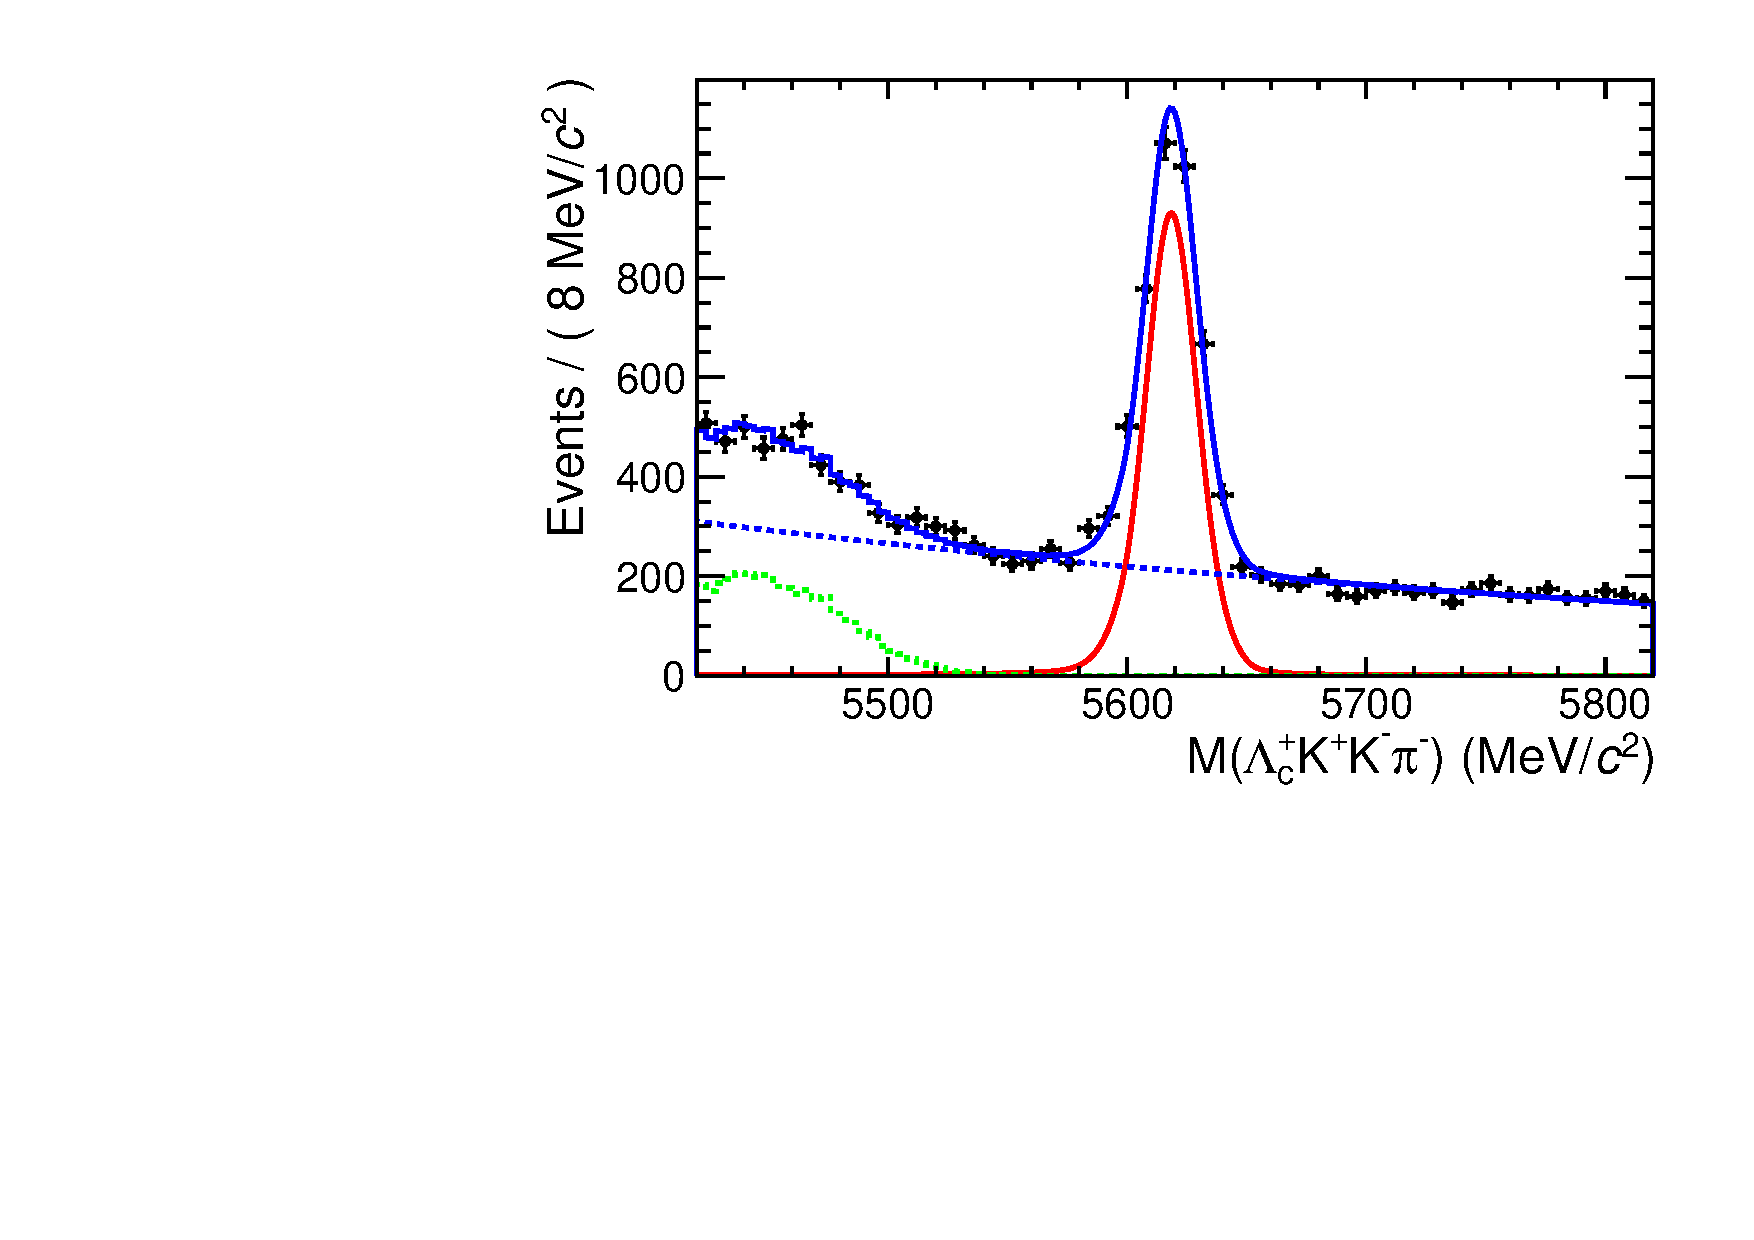
\includegraphics[width=0.5\textwidth]{Figures/05_open_charm/systematic/signal_model/Lb_LcKKPi.pdf}%
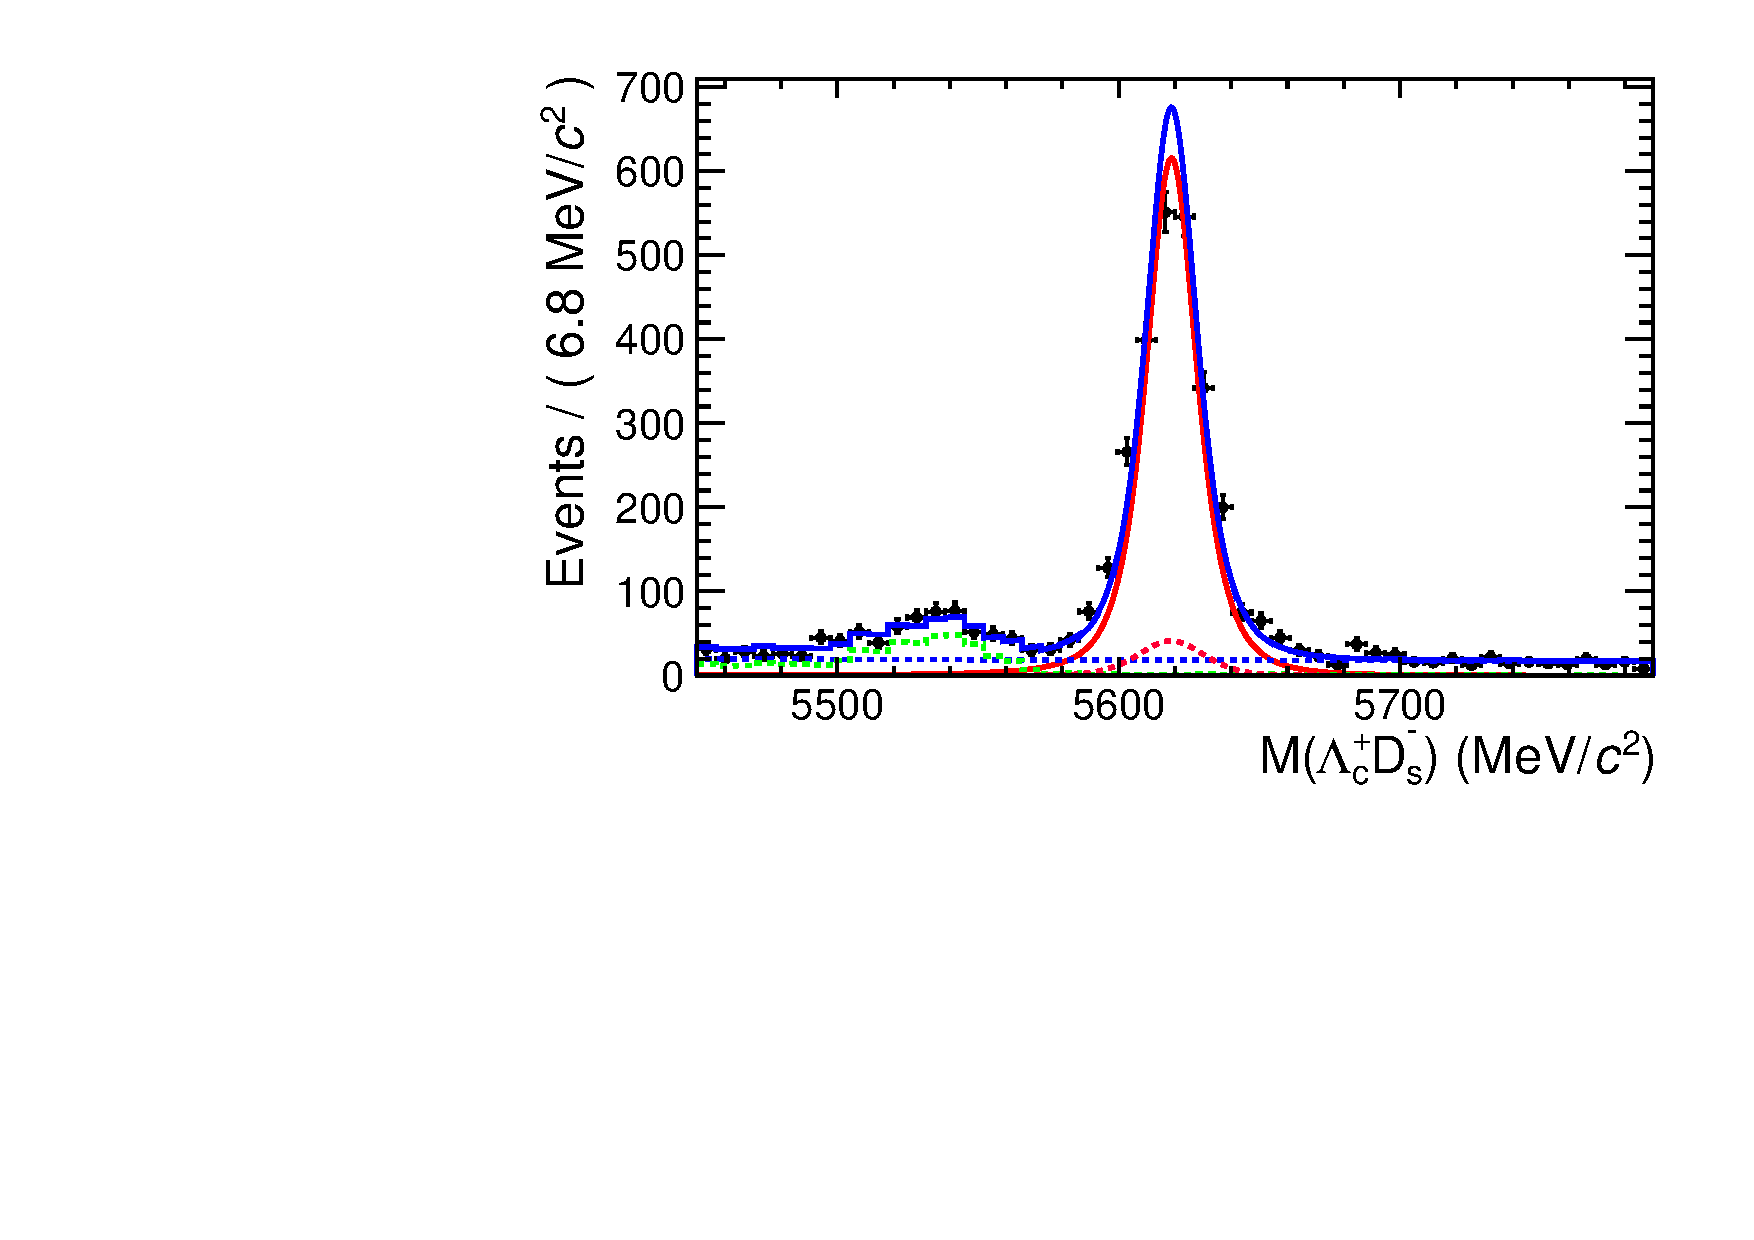
\includegraphics[width=0.5\textwidth]{Figures/05_open_charm/systematic/signal_model/Lb_LcDs.pdf}\\%
\caption{Invariant mass distributions for the \LbLckkpi sample(left) and \LbLcDs sample(right) with fit and residuals. 
The signal shape is described by Hypatia function and background shape is the nominal one.  
   The blue line is full fit, 
   the blue dashed line is the combinatorial background, 
   the red line is the signal shape, 
   the pink dashed line is \LbLckkpi background. }
\label{fig:signalmodel}
\end{figure}



\subsection{MC statistics}
\label{sec:mcstat}
The limited statistics of the simulated samples used to estimate efficiencies is considered as a source of systematic uncertainty, 
which can be calculated as the standard deviation of a binomial distribution:
\begin{equation}
\sigma_{\epsilon} = \sqrt{\epsilon(1-\epsilon)/N}
\end{equation}
where $\epsilon$ is the efficiency obtained from simulated events, 
and N stands for the total number of simulated events.
This expression should be modified if each event has different weights, 
which is due to the reweight mentioned in Sec.~\ref{sec:tuningMC}.

The statistic uncertainty of $\epsilon$ is
\begin{equation}
\sigma_{\epsilon} = \frac{\sqrt{\sum_i \epsilon_i(1-\epsilon_i) w_i^2}}{\sum_i  w_i },
 \end{equation}
where the $w_i$ is the weight for every event. This uncertainty is about 2.48\%.


\subsection{$\pt, ~y$ and nTracks reweight}
\label{sec:ptyweight}
The data and MC sample that we used to obtain the $\pt, ~y$ and nTracks weights have finite statistic, 
which leads to an uncertainty of each single-event weight.
A toy MC is used to propagate these uncertainties of single-event weights to the uncertainty of relative efficiency.
For each toy experiment, all the weights are varied randomly according to their errors, 
then the relative efficiency is evaluated.
The toy tests result in a distribution of the relative efficiency, 
whose RMS is taken as uncertainty for the relative efficiencies.
The systematic uncertainty is around 0.65\% according to the toy study.

Another source of systematic uncertainty about the reweight is from the binning scheme of the weight table. 
We rebin the $\pt, ~y$ table and calculate the relative efficiency of TOS lines again, 
the difference is taken as the systematic uncertainty of this source.
The corresponding uncertainty is around 0.43\%.
The similar method is applied to the nTracks reweight, and the corresponding result is 0.84\%.


\subsection{Dalitz reweight}
\label{sec:dalitz}

Toy experiments are used to study the uncertainty due the finite data and MC sample size. 
For each experiment, 
all the weights are varied randomly according to their errors, 
then the relative efficiency is evaluated. 
The toy tests result is a distribution of the relative efficiency, 
whose RMS is taken as uncertainty for the relative efficiencies.
The estimated uncertainty is around 1.12\%.

Another uncertainty source is the binning scheme of these two weight, 
we rebin the weight table randomly and recalculate the relative efficiencies, 
the difference between the new result and the default result as the systemic error from this source. 
This uncertainty is about 0.79\%.

\subsection{Trigger efficiency}

The L0 Hardron TOS trigger efficiency is gained from efficiency tables, 
with error bar in every bin. 
We generate many similar table according to the value and error of bins, 
then the relative efficiency is evaluated. The toy tests result is a distribution, 
and we take the RMS as the uncertainty. 
This uncertainty is about 0.09\%.


\subsection{PID efficiency}
\label{sec:pideff}
The PID efficiency is obtained using a data driven method, 
and the finite statistic of the calibration samples leads to uncertainty of the PID efficiencies. 
The \texttt{PIDCALIB} package gives the 3-D histograms that shows the single-event PID efficiency as well as its uncertainty.  
A toy Monte Carlo method is applied to propagate these uncertainties to the average PID efficiency. 
The PID efficiencies of each tracks are set to be a random number with the Gaussian distribution $G(\epsilon_{PID}, \sigma_{PID})$, 
where $\epsilon_{PID}$ stands for the value of PID efficiency from \texttt{PIDCALIB} package, 
and $\sigma_{PID}$ stands for the uncertainty.Due to lack of statistics in some bins of the efficiency tables.


\texttt{PIDCALIB} package sometimes gives unphysical efficiencies, 
which are smaller than zero, or larger than one. 
In the default treatment, 
we set negative PID efficiency as 0 and that larger than one as 1. 
So we estimate the systematic uncertainty of setting the larger 1 as 1. 
These efficiencies are replaced by uniform distribution random numbers ranged from 0 to 1. 
A new relative efficiencies are calculated with the same method and the differences are set to be the uncertainties.

Another source of systematic uncertainty about PID efficiency is from the binning scheme of the efficiency table, 
which is estimated by halve the bin size of momentum for all the particles. 
After this process, 
we find the relative efficiency get a negligible change, so we neglect this source here.
The PID uncertainty is about 0.4\%.

\subsection{$\Lc\pi$, $\Kp\Km$ and $\Lc\Kp\Km$ mass inconsistency and \Lb IP smearing}
\label{sec:sys_resonance}

Figure.~\ref{fig.Resonance_2body} and Figure.~\ref{fig.Resonance_3body} show the comparison between some invariant mass distributions 
in data after background subtraction with the Splot technique and the MC sample generated by phase-space model. 
We see significant difference between data and the background subtracted data in the invariant mass distribution of $\Lc\pi^-$. 
We apply a weight to the MC sample make it has same distribution with data sample in $\Lc\pi$ spectrum. 
This uncertainty is about 1.33\%.

Besides, 
we also find that the mass distributions of $\Kp\Km$ and $\Lc\Kp\Km$ are also inconsistent between the data and MC samples.
In this case, 
we apply a weight to the MC sample according to the $\Kp\Km$ distribution, 
then to estimate the efficiency again, and this uncertainty is about 2.62\%.
Then we use the same method to estimate the effect from the $\Lc\Kp\Km$ inconsistency between the data and MC smaples, 
and this uncertainty is about 2.03\%.
It is not reasonable to add these two uncertainties to the final results both, 
and we take the larger one as the uncertainty caused by the $\Kp\Km$ and $\Lc\Kp\Km$ distribution inconsistency.

We remove \Lb IP smearing and repeat all processes to recalculate the efficiency, 
and the difference are set to be the uncertainty. This uncertainty is about 0.09\%.



\subsection{Physical background effect }
\label{sec:sys_physical}
We change the mass region begins from $5500 \mev$ in \LbLckkpi fitting to exclude the partial reconstructed background in the low mass sideband, 
and take the yield difference as one systematic uncertainty. 
This uncertainty is about 0.26\%.

\begin{figure}[hbt]
\centering
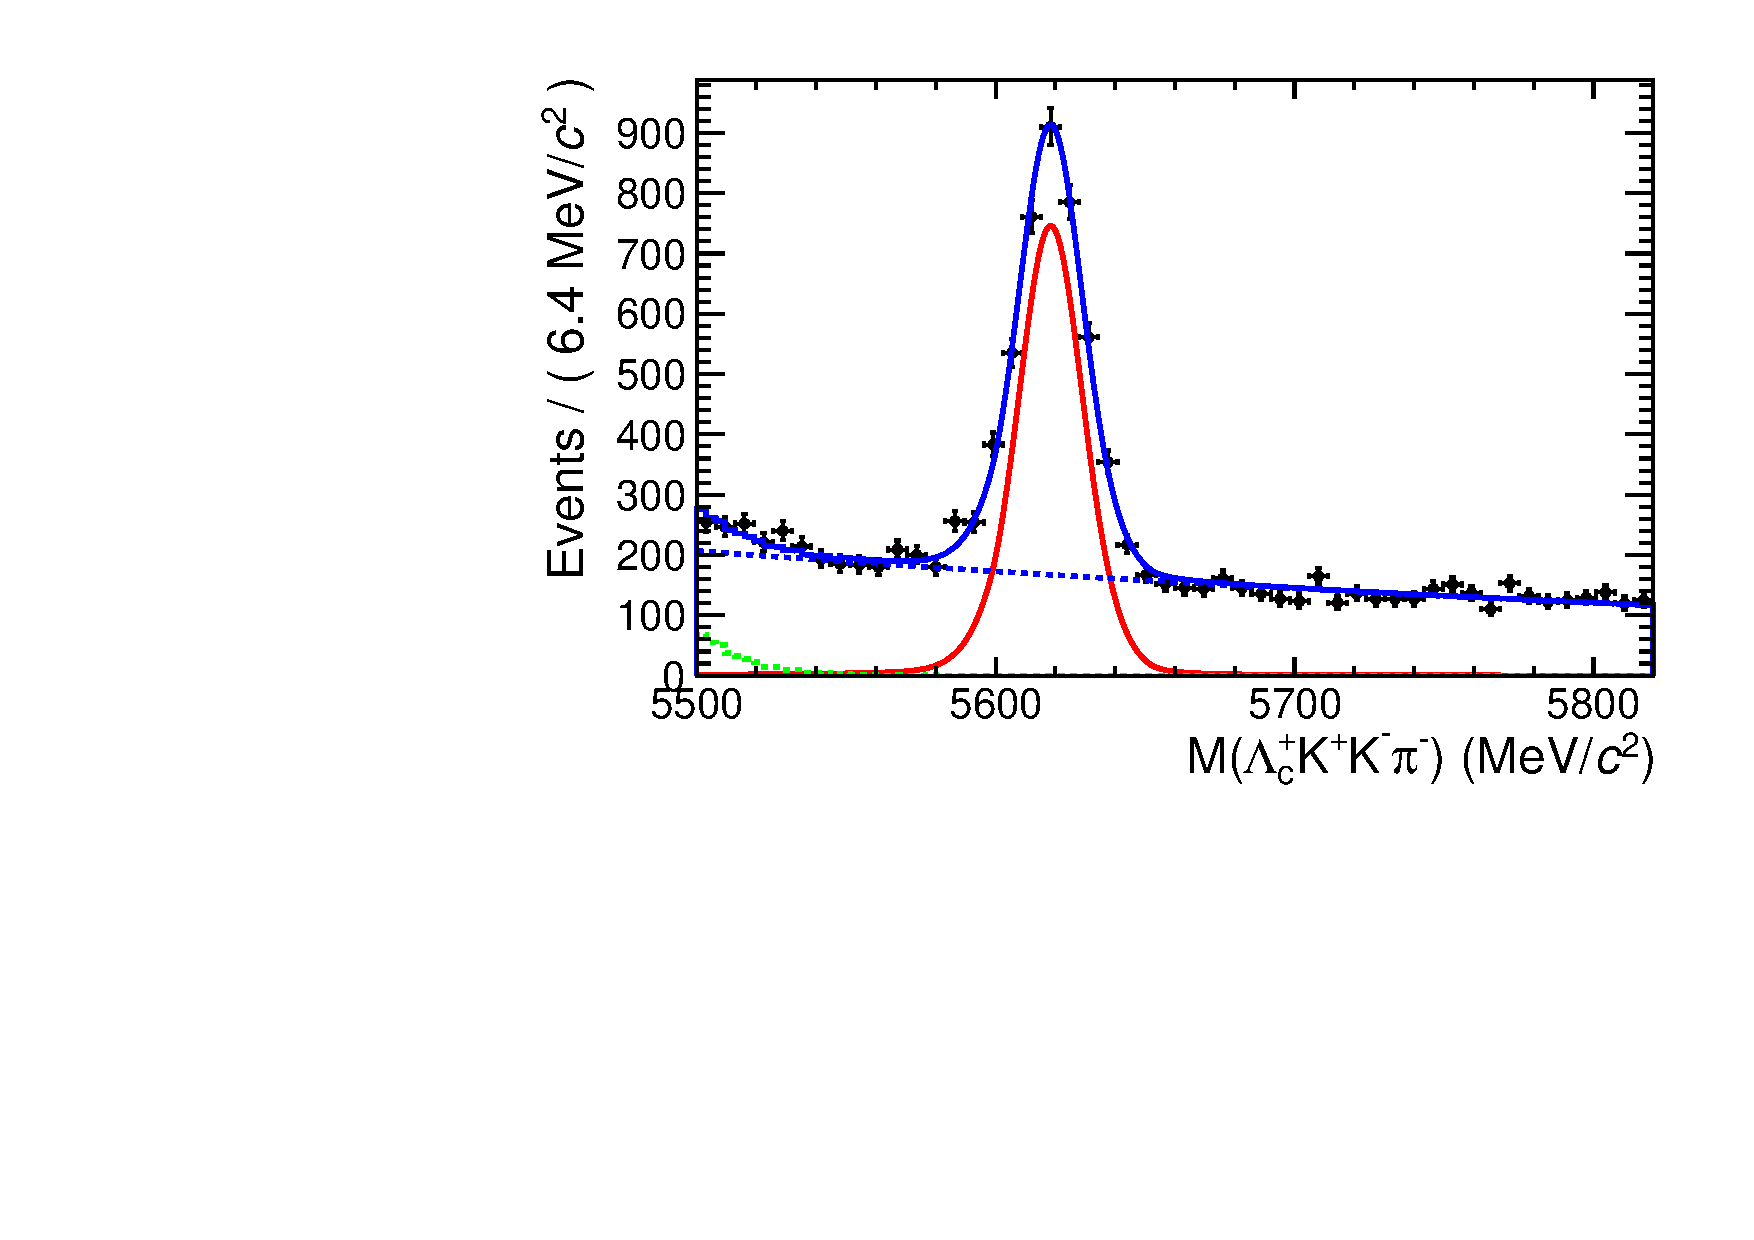
\includegraphics[width=0.5\textwidth]{Figures/05_open_charm/systematic/change_region/Lb_LcKKPi.pdf}%
\caption{Invariant mass distributions for the \LbLckkpi sample. 
The blue line is full fit, the blue dashed line is the combinatorial background, the red line is the signal shape. }
\label{fig:change_region}
\end{figure}


\subsection{ \LbLckkpi in normalization channel }
\label{sec:sys_Lckkpi_number}
When we estimate the yields of \LbLcDs, 
the number of \LbLckkpi backgound is fixed to value obtained from sideband.
In order to consider this uncertainty, 
we float the number of \LbLckkpi within the margin of error and fit mass distribution again.
The difference of the signal yield is considered as the systematic uncertainty.
This uncertainty is about 0.77\%.


\subsection{Fraction of different MC sample}
\label{sec:MC_fitting}

As we mixed three kinds of MC samples of \LbLckkpi channel together to estimate the efficiency, 
and the fraction is obtained by fitting the two dimentional distributions of $\Kp\Km\pim$ and $\Kp\pim$.
The fitting result is shown in the Figure.~\ref{Fig.Projection}, 
and the corresponding numbers are listed in Tab.~\ref{tab:MassFit_component}.
Then we studied the effect of the fraction used in the \LbLckkpi channel efficiency calculation.
We change the number of different MC sample according to their errors independently, 
and recalculate the final efficiency, 
and find the corresponding uncertainties are 0.016\%, 0.163\% and 0.028\%, 
this uncertainty is pretty small, 
and the total value is around 0.17\%.




